\section{Cryptographic Strength of S-Boxes}
The cryptographic strength of S-boxes is often measured using Boolean functions. 
A Boolean function is a function $f : \mathbb{F}_2^n \to \mathbb{F}_2 : GF(2^n) \to GF(2)$ \cite{Cusik09-1}.
For convenience, let $\Omega_n$ be the set of all Boolean functions on $n$ variables. Clearly,
we have that $|\Omega_n| = 2^{2^{n}}$. For all Boolean functions $f \in \Omega_n$ there exists a
unique truth table (TT) or Algebraic Normal Form (ANF) representation. The TT for a Boolean function
$f$ is simply the vector $(f(\bar{0}), \dots, f(\bar{1}))$, where each element corresponds to an element in $GF(2)$. 
The TT representation of Boolean functions offers a simple way to measure the distance between two
Boolean functions $f$ and $g$, since we can simply compute the Hamming distance between them.

Alternatively, we can represent Boolean functions as polynomials in $\mathbb{F}_2[x_0,\dots,x_{n-1}]/(x_0^2 - x_0,\dots,x_{n-1}^2 - x_{n-1})$,
which corresponds to their ANF representation. The process of translating a Boolean function $f$ to its ANF representation
is called the algebraic normal transform, and is defined as follows:
\begin{align*}
f(\bar{x}) = \sum_{i = (i_0,\dots,i_n) \in \mathbb{F}_2^n}a_ix_0^{i_0}x_1^{i_1}\dotsb x_{n-1}^{i_{n-1}} (\text{mod 2}),
%f(\bar{x}) = \bigoplus_{a_0,\dots,a_{n-1}} h(a_0,\dots,a_{n-1})x_0^{a_0} \dots x_{n-1}^{a_{n-1}} = \bigoplus_{\bar{a} \in GF(2^n)} h(\bar{a})\bar{x}^{\bar{a}}
\end{align*}
where $a_i \in \mathbb{F}_2$. S-boxes of the form $F : GF(2^n) \to GF(2^m)$ are unique Boolean functions in that they combine 
the output of $m$ individual Boolean functions in its output. In other words, they 
can be represented as a vector of $m$ Boolean functions $f_i, 1 \leq i \leq m$, that share the same
$n$ input bits, denoted as:
\begin{align*}
f_1(x_1,\dots,x_n) \\
f_2(x_1,\dots,x_n) \\
\vdots \\
f_{m-1}(x_1,\dots,x_n) \\
f_m(x_1,\dots,x_n)
\end{align*}
Based on this definition, we let $F(x) = (f_1(x),\dots,f_m(x))$. Boolean functions of this
type are called vectorial Boolean functions, and we denote them as $F : GF(2^n) \to GF(2)^m$
or $(n,m)$ S-boxes.

Cryptographically significant properties such as nonlinearity, resiliency, and algebraic immunity 
can be measured for a given Boolean function. These measurements are indications of the 
S-boxes susceptibility to linear cryptanalysis, statistical correlation, and algebraic attacks.
Another important property for these S-boxes is differential uniformity, first popularized in
terms of S-boxes by Nyberg in \cite{Nyberg94-1}. It is critically important to examine all
such measurements in the study and development of cryptographically strong S-boxes.

% Another common means of generating the ANF 
% representation is to construct the polynomial which consists of the sum of the polynomial
% $(a_0 \oplus a_0 \oplus 1)\dots(x_{n-1} \oplus a_{n-1} \oplus 1)$ for all $\bar{a} \in GF(2^n)$ such that $f(\bar{a}) = 1$. 
% This definition can be described as the following.
% \begin{align*}
% ANF(\bar{x}) = &  a_0 \oplus \\
% &  a_1x_1 \oplus ... \oplus a_{n}x_{n} \oplus \\
% &  a_{1,2}x_1x_2\oplus ... \oplus a_{n-1, n}x_{n-1}x_n \oplus \\
% &  ... \\
% &  a_{1,2,...,n}x_{1}...x_{n}
% \end{align*}

\subsection{Nonlinearity}
Since Boolean functions are natural representations for S-boxes, the measure of nonlinearity becomes
fundamental in the assessment of the cryptographic strength of S-boxes. For a Boolean function $f$,
we define the nonlinearity $\nl$ as follows:
\begin{align*}
\nl = \min_{\phi \in \mathcal{A}_n} d(f, \phi),
\end{align*}
where $\mathcal{A}_n$ is the set of all Boolean affine functions on $n$ variables, 
and $d(f, g) = wt(f \oplus g)$ (i.e. the Hamming distance between two functions $f$ and $g$) \cite{Cusik09-1}. 
Cryptographically strong S-boxes have high measures of nonlinearity, meaning that
it is increasingly difficult to approximate them using linear affine functions.
Subsequently, high measures of nonlinearity help hinder linear cryptanalysis attacks. 

\subsection{Resiliency}
Resiliency combines the measurements of balancedness and correlation immunity. 
Balancedness is a simple property of Boolean functions that captures the distribution of their output.
In particular, a Boolean function is balanced if its (Hamming) weight is $2^{n - 1}$. 
A Boolean function $f$ on $n$ variables is said to have a correlation immunity 
of order $t$, $1 \leq t \leq n$, if the output is statistically independent for any fixed subset of at most $t$ 
variables. In other words, given $f(\bar{x})$, the probability that $t$ fixed input variables have 
any set of values is always $2^{-t}$. Correlation immunity is an important property of 
cryptosystems with the advent of correlation attacks on stream ciphers \cite{Canteaut05-1}.
A higher correlation immunity indicates a lower susceptibility to such attacks.

\subsection{Algebraic Immunity}
This metric is used to determine a Boolean functions resilience to attacks
based on annihilators \cite{Cusik09-1}. Formally, an annihilator of a Boolean 
function $f$ is another a Boolean function $g$ such that $f \oplus g = 0$. 
Using low-degree annihilators it is sometimes possible to reduce the degree
of a Boolean function to a small enough value such that the system of 
equations relating the Boolean function and state or key bits of a cryptosystem
can be solved in a reasonable amount of time \cite{Frederik04-1}. 

\subsection{Differential Uniformity}
Differential uniformity relates to the S-boxes resistance to differential cryptanalysis
attacks. First introduced in 1994 by Nyberg \cite{Nyberg94-1}, we say that
an S-box $F : GF(2^n) \to GF(2^m)$ is $\delta$-differentially uniform if for all $\alpha \in GF(2^n)$
and $\beta \in GF(2^m)$ we have
\begin{align*}
|\{x \in GF(2^n) | F(x + \alpha) = \beta\}| \leq \delta.
\end{align*}
Differential cryptanalysis exploits the lack of uniformity in the nonlinear S-box
step of SPN block ciphers. Cryptographically strong S-boxes have low values for
$\delta$, as this means the output of $F$ is relatively uniform and the frequency of a 
single output value cannot be easily exploited for an attack. 
Differential uniformity was first studied in the context of the Data Encryption
Standard, and it was proven in \cite{Nyberg94-1} that if the round functions of
Feistel-based ciphers similar to DES are $\delta$-differentially uniform, then 
the average probability to obtain a non-zero output for input $x + \alpha$, for
all $x, \alpha \in GF(2^n)$, after a fixed number of rounds is bounded by $2(\frac{\delta}{2^n})^2$.

S-boxes of the form $F(x) : x^{-1}$ were shown to be $4$-differentially uniform 
with a $\nl$ lower bound of $2^{n-1} - 2^{\frac{n}{2}}$ in \cite{Nyberg94-1}.
Similarly, S-boxes of the form $F(x) = x^{2^{k} + 1}$ are $2$-differentially uniform
with a $\nl$ equal to precisely $2^{n-1} - 2^{\frac{n-1}{2}}$. With the selection
of Rijndael as the AES in 2001 \cite{Daemen02-1}, S-boxes of the form $F(x) : x^{-1}$
became the primary subject of study in the literature. 

% TODO: normal basis implementation for efficient squaring of this power mapping? YES PLEASE!

\subsection{Construction Techniques}
Constructing cryptographically significant Boolean functions is a well-studied problem
in the literature. For the purposes of this work, we restrict ourselves to a 
single class of Boolean function constructions belonging to the Maiorana-McFarland
class of functions, which are used to construct bent functions \cite{Gupta05-1, Gupta02-1}. 
These construction techniques can be used to build $(n,m,t)$ resilient S-boxes with
degree $d > m$. Efficient software implementations of similar functions are
presented in \cite{Gupta02-1}. Furthermore, as Boolean functions, the output of these
constructions can be directly mapped to combinational logic and implemented in hardware. 

%http://arxiv.org/pdf/1003.3492v1.pdf

\section{Techniques for Efficient Implementations}
Computing the multiplicative inverse of elements in $GF(2^k), k = nm,$ is a long-studied
problem dating back to the early 1990s \cite{Brunner93-1}. At the time, computing
inverses using Fermat's theorem or the Extended Euclidean algorithm were popular 
techniques. Modern approaches for minimizing the circuit complexity of the multiplicative inverse step
rely on composite field arithmetic to reduce the operations
to elements in smaller fields. Such decompositions often rely on a change in basis between
two fields, where the change is between polynomial and normal bases.
We discuss recent work of both schemes in the following sections.

\subsection{Composite Field Representations for Inverses}
A \emph{composite field} is a pair $\{GF(2^n), Q(y) = y^n + \sum_{i=0}^{n-1}q_iy^i, q_i \in GF(2)\}$ and
$\{GF((2^n)^m), P(x) = x^m + \sum_{i=0}^{m-1}p_ix^i, p_i \in GF(2^n)\}$ where $GF(2^n)$ 
is constructed from $GF(2)$ by $Q(y)$, and $GF((2^n)^m)$ is constructed from 
$GF(2^n)$ by $P(x)$. We state that $GF((2^n)^m)$ is a degree $m$ extension of $GF(2^n)$.
This form of extension means that the coefficients of the polynomials in $GF((2^n)^m)$
are themselves elements of $GF(2^n)$. 

Using composite field arithmetic, it is possible to reduce the multiplicative
inverse calculation of elements $a \in GF(2^k)$ to calculations in $GF((2^n)^m)$.
In particular, given a composite field $GF((2^n)^m)$, where $m = 2$ and $P(x) = x^2 + Ax + B$,
there exists a decomposition from $GF(2^k)$ to $GF((2^n)^m)$. With such a
decomposition, we can now compute $a^{-1}$ as follows:
\begin{align}
a^{-1} = (bx + c)^{-1} = b(b^2B + bcA + c^2)x^{-1} + (c + bA)(b^2B + bcA + c^2)^{-1},
\end{align}
\begin{figure}[ht!]
\begin{center}
	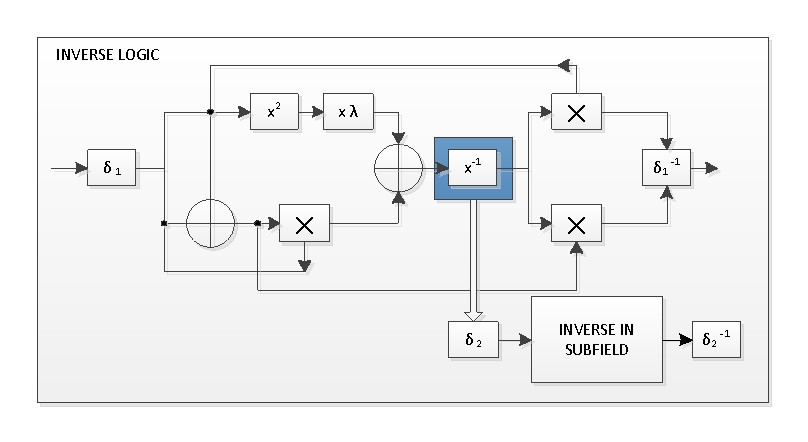
\includegraphics{images/composite_field_inverter.pdf}
\end{center}
\caption{Multiplicative inverse calculation using composite field decomposition. The blocks $\delta_1$ and
$\delta_1^{-1}$ are constant multiplications with the basis transformation matrices from $GF(2^k)$ to
$GF((2^n)^m)$, respectively. }
\label{fig:compositeFieldInverse}
\end{figure}
The circuitry required to implement this calculation is shown in Figure \ref{fig:compositeFieldInverse}. 
Since $b, c, B, A \in GF(2^n)$, we can recursively decompose the inverse of $(b^2B + bcA + c^2)$ into
elements of the field $GF(2^{n/2})$ (assuming $GF(2^n)$ can be represented as a degree $2$ extension
of the field $GF(2^{n/2})$). Such designs are referred to as tower field decompositions. Satoh et al.
explored all tower field decompositions for $GF(2^8)$ in \cite{Satoh01-1}. The field extensions they 
used are shown below, where $\phi \in GF(2^2)$ and $\lambda \in GF((2^2)^2)$ are chosen such that $P(x)$
is irreducible over their respective extension fields.
\begin{align*}
GF(2) \to GF(2^2)\text{ , }& P(x) = x^2 + x + 1 \\
GF(2^2) \to GF((2^2)^2)\text{ , }& P(x) = x^2 + x + \phi \\
GF((2^2)^2) \to GF(((2^2)^2)^2)\text{ , }& P(x) = x^2 + x + \lambda 
\end{align*}
To convert between elements in $GF(2^k)$ and $GF((2^n)^m)$ represented in 
a polynomial basis, where $k = nm$, it is necessary to find a mapping between 
these two fields such that additive and multiplicative homomorphism is maintained. 
A polynomial basis for a field $GF(2^k)$ defined by a primitive irreducible polynomial $P(x)$
and primitive element $x$ is the set $\{x^{k-1}, \dots,x^2,x,1\}$. Each element
in this basis is linearly independent from all others, so it is possible to represent every element
in the field using this basis. In addition, the basis element $x$ can 
be used to generate every element in the field $GF(2^k)$ as $\{0, 1, x,\dots, x^{p^{k} - 2}\}$.
By finding two primitive elements $\alpha \in GF(2^k)$ and $\beta \in GF((2^n)^m)$, 
the mapping $\alpha^i \to \beta^i, 0 \leq i \leq 2^k - 1$ can then be defined 
by mapping the basis $\alpha$ of $GF(2^k)$ to the basis $\beta$ of $GF((2^n)^m)$.
The result is a binary $k \times k$ matrix \textbf{T} such that \textbf{T}$\alpha^i = \beta^i$.
This matrix can be defined by \textbf{T}$ = [(\beta^0)^T, (\beta^1)^T,\dots,(\beta^{k-1})^T]$.
The transformation matrix \textbf{T} and its inverse \textbf{T}$^{-1}$ used by Satoh et al.
are shown below.
\begin{align*}
	\text{\textbf{T}} =  \left( \begin{array}{cccccccc}
1 & 1 & 0 & 0 & 0 & 0 & 1 & 0 \\
0 & 1 & 0 & 0 & 1 & 0 & 1 & 0 \\
0 & 1 & 1 & 1 & 1 & 0 & 0 & 1 \\
0 & 1 & 1 & 0 & 0 & 0 & 1 & 1 \\
0 & 1 & 1 & 1 & 0 & 1 & 0 & 1 \\
0 & 0 & 1 & 1 & 0 & 1 & 0 & 1 \\
0 & 1 & 1 & 1 & 1 & 0 & 1 & 1 \\
0 & 0 & 0 & 0 & 0 & 1 & 0 & 1 \end{array} \right) \hspace{2em} \text{\textbf{T}}^{-1} = 
\left( \begin{array}{cccccccc}
1 & 0 & 1 & 0 & 1 & 1 & 1 & 0 \\
0 & 0 & 0 & 0 & 1 & 1 & 0 & 0 \\
0 & 1 & 1 & 1 & 1 & 0 & 0 & 1 \\
0 & 1 & 1 & 1 & 1 & 1 & 0 & 0 \\
0 & 1 & 1 & 0 & 1 & 1 & 1 & 0 \\
0 & 1 & 0 & 0 & 0 & 1 & 1 & 0 \\
0 & 0 & 1 & 0 & 0 & 0 & 1 & 0 \\
0 & 1 & 0 & 0 & 0 & 1 & 1 & 1 \end{array} \right)
\end{align*}
The complexity of the S-box calculation is based on the transformation matrix used to map every element
$\alpha \in GF(2^k)$ to an element $\beta \in GF((2^n)^m)$, as well as the constant multiplication 
operations in the multiplicative inverse block, both of which depend on the choice of
irreducible polynomials for $P(x)$. Rudra et al. \cite{Rudra01-1} present functions for
estimating the gate complexity of an S-box given the field representations. Once optimized solutions for the
gate complexity are found, the Boolean logic for the transformation matrices can be further
simplified using a greedy compression algorithm, as presented in \cite{Morioka99-1}.
Mentens et al. \cite{Mentens05-1} examined the composite field definitions and corresponding
S-box used by Satoh et al. and showed that their results were 5\% away from an optimal solution.
This was determined by choosing a different constant $\lambda = \{1000\}_2$ such that the 
base field multiplication operation in (1) contains one additional XOR gate with the benefit
of reducing the complexity of the transformation matrix \textbf{T} by 5 gates.

\subsection{Normal Basis Transformations}
The normal basis for a finite field $GF(2^k)$ is defined as the set $\{\beta, \beta^2, \beta^{2^2},\dots,\beta^{2^{k-1}}\}$, 
where $\beta \in GF(2^k)$ and all elements in the set are linearly independent. An immediate result of representing
elements using the normal basis of a field is that squaring comes for free in hardware (i.e. it equates to a bit-wise
rotation of the element). For this reason, composite field decompositions using normal bases, rather than polynomial
bases, have been another popular topic of research in the literature \cite{Nikova08-1, Canright05-1}.

When the multiplicative inverse calculation is decomposed into operations on smaller fields
represented in a normal basis, multiplication and inversion in the base field are still the most expensive procedures of the 
entire calculation. With this basis representation, the multiplicative
inverse operation can be expressed in very elegant equations, as shown in \cite{Nikova08-1}. 
For both of these operations, let $ax + b$ and $cx + d$ be two elements in $GF((2^n)^m)$,
and let $\{v,m v^l\}$ be a normal basis of $GF((2^n)^m)$. The product of these
two elements is $ex + f = (ax + b) \times (cx + d)$, where $e = (a + b)(c + d)g + ac, f = (a + b)(c + d)g + bd$ and 
$g = v^2 + v$ (the trace of $v$ over $GF(2^n))$. Similarly, the inverse $(ax + b)^{-1}$ can be defined
as $(cx + d) = (ax + b)^{-1}$, where $c = ((a + b)^2g + ab)^{-1}b$ and $((a + b)^2g + ab)^{-1}a$.
Again, the inverse operation requires one to calculate the inverse of elements over $GF(2^n)$,
and so this process can be repeated recursively. Alternatively, the inverse of elements in $GF(2^n)$ 
may be optimized using Boolean function minimization based on its ANF representation, as is done in \cite{Nikova08-1}. 

%\subsection{Fermat's Theorem for Inverse}
%TODO: inverse and derivation here (and comment about rotation)
%\subsection{Normal Basis}
%TODO: describe how normal basis works and why squaring is free